\documentclass[a4j]{jsarticle}

\usepackage{enumerate}
\usepackage{amsmath,amssymb}
\usepackage[dvipdfmx]{graphicx}
\usepackage{array}
\usepackage{float}
\usepackage{amsmath}
\usepackage{listings,jlisting}
\usepackage{ascmac}
\usepackage[dvipdfmx]{graphicx}
\usepackage{subcaption}
\usepackage{slashbox}
\usepackage{subcaption}
\usepackage{textcomp}
\usepackage{multirow}
\usepackage{itembkbx}
\usepackage{color}
\usepackage{url}
\lstset{language=ruby,numbers=left,frame=tlrb,basicstyle=\ttfamily,commentstyle=\ttfamily,breaklines=true,breakindent = 40pt,lineskip=-0.2ex,tabsize = 2,showstringspaces=false,classoffset = 0,frame = tlBR,backgroundcolor={\color[gray]{.90}}}
%,backgroundcolor={\color[gray]{.90}}
\usepackage{listings,jlisting}
\usepackage[top = 27truemm, bottom = 35truemm, left = 27truemm, right = 27truemm]{geometry}
%\renewcommand{\labelenumi}{(\alph{enumi})}
\usepackage{mdframed}
\def\WordCount#1{%
  \@tempcnta\z@
  \@tfor \@tempa:=#1\do{\advance\@tempcnta\@ne}%
  \the\@tempcnta
}
\makeatletter
\def\lst@lettertrue{\let\lst@ifletter\iffalse}
\makeatother
%%%%%  箇条書きの設定   %%%%%
\renewcommand{\labelitemi}{$\triangleright$}
\renewcommand{\labelenumi}{(\arabic{enumi}).}

%%%%%%%%%%%%%%%%%%%%%%%%%%%%%%%%%%%%%%%%%%%%%%%%%%%%%%%%%%%%%%%%%%%%%%%%%%%%%
\begin{document}

\begin{titlepage}
\begin{center}
\vspace*{230truept}
\huge{4Jシミュレーション}\\
\huge{レポート3}\\
\vspace*{30truept}
\Large{4年 電子情報工学科 9番 \\岡村宙輝}\\
\vspace*{50truept}
\Large{2019年 2月 19日(火) 提出}\\
\end{center}
\end{titlepage}

\newgeometry{top = 20truemm,, bottom = 35truemm, left = 27truemm, right = 27truemm}

%%%%%%%%%%%%%%%%%%%%%%%%%%%%%%%%%%%%%%%%%%%%%%%%%%%%%%%%%%%%
\section{目的}
ガウスの消去法を使ったプログラムを用いて,連立一次方程式が解けるようになる.
さらに,ガウスの消去法を使って最小二乗法による直線,曲線近似を行うプログラム
を作成する.このプログラムを利用し,データを近似した1次多項式の傾きと切片,
,2次多項式の係数などを求める.

%%%%%%%%%%%%%%%%%%%%%%%%%%%%%%%%%%%%%%%%%%%%%%%%%%%%%%%%%%%%
\section{実行環境}
実行環境を表\ref{kan}に示す.

\begin{table}[htbp]
\begin{center}
\caption{実行環境}
\label{kan}
\begin{tabular}{|c|l|}
\hline
CPU&Intel(R)Core(TM) i7-4500U CPU @ 1.80GHz 2.4GHz \\
\hline
メモリ&8.00GB\\
\hline
OS&Ubuntu 16.04.5 LTS\\
\hline
言語&Python3,C\\
\hline
コンパイラ&gcc 5.4.0\\
\hline
\end{tabular}
\end{center}
\end{table}


%%%%%%%%%%%%%%%%%%%%%%%%%%%%%%%%%%%%%%%%%%%%%%%%%%%%%%%%%%%%
\section{課題9:ガウスの消去法}
連立方程式を解くための,ガウスの消去法と呼ばれる方法を用いる.
ガウスの消去法では大きくわけて前進消去と後退代入の2つの手順がある\cite{sim}.
\begin{eqnarray}
\begin{cases}
x_1  + 2x_2 = 10\\
3x_1 + 4x_2  = 15\\
\end{cases}
\label{gaus}
\end{eqnarray}

式(\ref{gaus})を解く場合,まず式(\ref{gaus2})のように変形して$A,b$を入力とする.
\begin{equation}
   A=\begin{pmatrix} 1 & 2 \\ 3 & 4 \end{pmatrix},b=\begin{pmatrix} 10 \\ 15 \end{pmatrix}
   \label{gaus2}
\end{equation}

前進消去のアルゴリズムを次に示す.$n$は$A$の次数を表しており,
式(\ref{gaus2})の場合は2である.$A$の$i$行$k$列目の値を$a_{ik}$と表す.
\begin{itemize}
 \item 各列$k=1,2,\ldots,n-1$について,次の処理を反復する.
       \begin{itemize}
	\item 各行$i=k+1,k+2,\ldots,n$について,次の処理を反復する.
	      \begin{enumerate}
	       \item{乗数$m \leftarrow a_{ik}/a_{kk}$}
	       \item $a_{ik} \leftarrow 0.(この代入は無くてもよい.)$
	       \item{各列$j=k+1,k+2,\ldots,n$について,
		    $a_{ij} \leftarrow a_{ij}-a_{kj}\times m$を反復する.}
	       \item{$b_i\leftarrow b_i - b_k \times m$}
	      \end{enumerate}
       \end{itemize}
\end{itemize}

前進消去を行った後は後退代入を行う.後退代入のアルゴリズムを次に示す.

\begin{itemize}
 \item 各行$k=n,n-1,\ldots,1$について,次の処理を反復する.
       \begin{enumerate}
	\item $x_k \leftarrow b_k$
	\item 各列$j=k+1,k+2,\ldots,n$について,$x_k \leftarrow x_k - a_{kj}\times x_j$
	      を反復する.
	\item $x_k\leftarrow x_k/a_{kk}$
       \end{enumerate}
\end{itemize}

%%%%%%%%%%%%%%%%%%%%%%%%%%%%%%%%%%%%%%%%
\subsection{課題9-1}
式(\ref{siki9-1})の連立方程式を解く.作成したプログラムをソースコード\ref{pro91}
に示す.

\begin{eqnarray}
  \begin{cases}
   2x + 2y + 6z = 24\\
   3x + 5y + 13z = 52\\
   5x + 8y + 24z = 93
  \end{cases}
  \label{siki9-1}
\end{eqnarray}

\lstinputlisting[caption=課題9-1のプログラム,label=pro91]{./program/kadai9/ichi.py}

実行結果を次に示す.
\begin{breakitembox}[l]{課題9-1の実行結果}
\begin{verbatim}

左辺:
[2, 2, 6]
[3, 5, 13]
[5, 8, 24]
右辺: [24, 52, 93]
前進消去後: [24, 16.0, 9.0]
後進代入後: [1.0, 2.0, 3.0]
\end{verbatim}
\end{breakitembox}

実行結果より,正しく計算できていることがわかる.

%%%%%%%%%%%%%%%%%%%%%%%%%%%%%%%%%%%%%%%%
\subsection{課題9-2}
式(\ref{siki9-2})の連立方程式をガウスの消去法プログラムで解き,
$x_1$〜$x_4$までの値を求める.
得られた解が連立方程式を満たすことを元の方程式に代入して確認する.
作成したプログラムをソースコード\ref{pro92}に示す.
\begin{eqnarray}
 \begin{cases}
  x_1  + 2x_2 + x_3  + 5x_4 = 20.5\\
  8x_1 + x_2  + 3x_3 + x_4  = 14.5\\
  x_1  + 7x_2 + x_3  + x_4  = 18.5\\
  x_1  + x_2  + 6x_3 + x_4  = 9.0
 \end{cases}
\label{siki9-2}
\end{eqnarray}

\lstinputlisting[caption=課題9-2のプログラム,label=pro92]{./program/kadai9/two.py}

実行結果を次に示す.
\begin{breakitembox}[l]{課題9-2の実行結果}
\begin{verbatim}

左辺:
[1, 2, 1, 5]
[8, 1, 3, 1]
[1, 7, 1, 1]
[1, 1, 6, 1]
右辺: [20.5, 14.5, 18.5, 9.0]
前進消去後: [20.5, -149.5, -51.83333333333333, -167.4]
後進代入後: [1.0000000000000036, 2.0, 0.4999999999999972, 3.0]
*****    検算   *****
1 * 1.0000000000000036 + 2 * 2.0 + 1 * 0.4999999999999972 + 5 * 3.0 = 20.50000
8 * 1.0000000000000036 + 1 * 2.0 + 3 * 0.4999999999999972 + 1 * 3.0 = 14.50000
1 * 1.0000000000000036 + 7 * 2.0 + 1 * 0.4999999999999972 + 1 * 3.0 = 18.50000
1 * 1.0000000000000036 + 1 * 2.0 + 6 * 0.4999999999999972 + 1 * 3.0 = 9.00000
\end{verbatim}
\end{breakitembox}

検算を行った結果より,正しく計算できていることがわかる.

%%%%%%%%%%%%%%%%%%%%%%%%%%%%%%%%%%%%%%%%%%%%%%%%%%%%%%%%%%%%
\section{課題10:ガウスの消去法(ピボット選択)}
前述したように前進消去のときには,乗数$m$に$a_{ik}/a_{kk}$を代入する.
このとき$a_{kk}$をピボットと呼び,ピボットが0である場合はエラーになってしまう.
このエラーを避けるために,絶対値を比較して行を入れ替えるピボット選択という処理
を行う.

%%%%%%%%%%%%%%%%%%%%%%%%%%%%%%%%%%%%%%%%
\subsection{課題10-1}
式(\ref{siki10-1})の連立方程式を解き,ピボット選択ありとなしで比較する.
作成したプログラムをソースコード\ref{pro101}に示す.

\begin{eqnarray}
 \begin{cases}
  -2x + 2y      = 0\\
  3x  - 3y +  z = 0\\
  2x  +  y + 6z = 0
 \end{cases}
 \label{siki10-1}
\end{eqnarray}
\lstinputlisting[caption=課題10-1のプログラム,label=pro101]
{./program/kadai10/kadai10-1.py}

実行結果を次に示す.
\begin{breakitembox}[l]{課題10-1の実行結果}
\begin{verbatim}
	
左辺:	
[-2, 2, 0]
[3, -3, 1]
[2, 1, 6]
右辺: [0, 1, 9]
*** ピボット選択あり ***
前進消去後: [1, 8.333333333333334, 0.6666666666666666]
後進代入後: [1.0000000000000002, 1.0000000000000002, 1.0]
*** ピボット選択なし ***
Traceback (most recent call last):
  File "kadai10-1.py", line 62, in <module>
    resultb, resultx = gaussian(A, b)
  File "kadai10-1.py", line 5, in gaussian
    m = A[i][k] / A[k][k]
ZeroDivisionError: float division by zero
\end{verbatim}
\end{breakitembox}

ピボット選択をしないと,0除算が発生してしまいエラーが出てしまうことがわかる.
ピボット選択をした場合は正しく計算できていることがわかる.
%%%%%%%%%%%%%%%%%%%%%%%%%%%%%%%%%%%%%%%%
\subsection{課題10-2}
式(\ref{siki10-2})の連立方程式をピボット選択を使って解き,
double型とfloat型で比較する.
作成したプログラムをソースコード\ref{pro102}に示す.
ソースコード\ref{pro102}のdoubleを全てfloatに変えれば,
float型で求めることができる.
\begin{eqnarray}
 \begin{cases}
  1.0x_1  + 0.96x_2   +   0.84x_3 +   0.64x_4 = 3.44\\
  0.96x_1 + 0.9214x_2 + 0.4406x_3 + 0.2222x_4 = 2.5442\\
  0.84x_1 + 0.4406x_2 +    1.0x_3 + 0.3444x_4 = 2.6250\\
  0.64x_1 + 0.2222x_2 + 0.3444x_3 +    1.0x_4 = 2.2066
 \end{cases}
 \label{siki10-2}
\end{eqnarray}
\lstinputlisting[caption=課題10-2のプログラム,label=pro102]
{./program/kadai10/cni.c}

実行結果を次に示す.
\begin{breakitembox}[l]{課題10-2の結果:double型}
\begin{verbatim}

A =
(1.0000000000  0.9600000000  0.8400000000  0.6400000000  )
(0.9600000000  0.9214000000  0.4406000000  0.2222000000  )
(0.8400000000  0.4406000000  1.0000000000  0.3444000000  )
(0.6400000000  0.2222000000  0.3444000000  1.0000000000  )
b =
(3.4400000000  2.5442000000  2.6250000000  2.2066000000  )
x =
(1.0000000000  1.0000000000  1.0000000000  1.0000000000  )
\end{verbatim}
\end{breakitembox}

\begin{breakitembox}[l]{課題10-2の結果:float型}
\begin{verbatim}

A =
(1.0000000000  0.9599999785  0.8399999738  0.6399999857  )
(0.9599999785  0.9214000106  0.4406000078  0.2222000062  )
(0.8399999738  0.4406000078  1.0000000000  0.3443999887  )
(0.6399999857  0.2222000062  0.3443999887  1.0000000000  )
b =
(3.4400000572  2.5441999435  2.6250000000  2.2065999508  )
x =
(0.9998441339  1.0001490116  1.0000523329  0.9999513030  )
\end{verbatim}
\end{breakitembox}

実行結果よりdouble型は$1\times10^{-10}$まで精度が出ている一方で,
float型は$1\times10^{-1}$から誤差が出ていることがわかる.
よってdouble型の方がfloat型より精度が高いことがわかる.

%%%%%%%%%%%%%%%%%%%%%%%%%%%%%%%%%%%%%%%%%%%%%%%%%%%%%%%%%%%%
\section{課題11:最小二乗法}
$n$個の座標$(x_1,y_1),(x_2,y_2),(x_3,y_3)\ldots(x_n,y_n)$を
通る関数$y=f(x)$を近似するために,最小二乗法という方法を使う.
最小二乗法では近似した式がすべての座標の点を通るということは考えず,
$n$個の座標と近似した式の違いが最小になるものを求める.
$n$個の座標$(x_1,y_1),(x_2,y_2),(x_3,y_3)\ldots(x_n,y_n)$のデータを
1次多項式$y=a+bx$で近似する場合は,式(\ref{kin1})で$a,b$を求めて近似を行う.
連立1次方程式を解くときには,ガウスの消去法を使用する.
\begin{eqnarray}
 \begin{cases}
  \begin{split}
   ma + \Bigl(\sum_{k=1}^{m} x_k\Bigr)b &= \sum_{k=1}^{m} y_k\\
   \Bigl(\sum_{k=1}^{m} x_k\Bigr)a + \Bigl(\sum_{k=1}^{m} {x_k}^2 \Bigr)b &= \sum_{k=1}^{m} x_ky_k
  \end{split}
 \end{cases}
 \label{kin1}
\end{eqnarray}

2次多項式$y=a+bx+cx^2$で近似する場合は,式(\ref{kin2})で$a,b,c$を求めて近似を行う.

\begin{eqnarray}
 \begin{cases}
  \begin{split}
   ma + \Bigl(\sum_{k=1}^{m} x_k\Bigr)b + \Bigl(\sum_{k=1}^{m} {x_k}^2\Bigr)c  &= \sum_{k=1}^{m} y_k\\
   \Bigl(\sum_{k=1}^{m} x_k\Bigr)a + \Bigl(\sum_{k=1}^{m} {x_k}^2 \Bigr)b + \Bigl(\sum_{k=1}^{m} {x_k}^3\Bigr)c &= 
   \sum_{k=1}^{m} x_ky_k\\
   \Bigl(\sum_{k=1}^{m} {x_k}^2\Bigr)a + \Bigl(\sum_{k=1}^{m} {x_k}^3\Bigr)b + \Bigl(\sum_{k=1}^{m} {x_k}^4\Bigr)c &=
   \sum_{k=1}^{m} {x_k}^2y_k
  \end{split}
 \end{cases}
 \label{kin2}
\end{eqnarray}




%%%%%%%%%%%%%%%%%%%%%%%%%%%%%%%%%%%%%%%%
\subsection{課題11-1}
表\ref{data111}のデータに対して最小二乗近似の1次多項式を求める.
作成したプログラムをソースコード\ref{pro111}に示す.
\begin{table}[H]
 \centering
 \caption{1次多項式近似のデータ}
\label{data111}
 \begin{tabular}{|c||c|c|c|c|}
  \hline
  i&1&2&3&4\\
  \hline
  \hline
  $x_i$&1&2&3&4\\
  \hline
  $y_i$&0&1&2&4\\
  \hline
 \end{tabular}
\end{table}

\lstinputlisting[caption=課題11-1のプログラム,label=pro111]
{./program/kadai11/one.py}

実行結果を次に示す.表\ref{data111}のデータと実行結果から得られた近似式
をプロットしたグラフを図\ref{graph11-1}に示す.
\begin{breakitembox}[l]{課題11-1の実行結果}
\begin{verbatim}
y = -1.5000000000000022 + 1.3000000000000007 x		
\end{verbatim}
\end{breakitembox}

\begin{figure}[htbp]
 \centering
 \includegraphics[scale=0.7]{res11-1.eps}
 \caption{課題11-1の実行結果:グラフ}
 \label{graph11-1}
\end{figure}

グラフより正しく近似できていることがわかる.

%%%%%%%%%%%%%%%%%%%%%%%%%%%%%%%%%%%%%%%%
\subsection{課題11-2}
表\ref{data112}のデータに対して,2次式$y=a+bx+cx^2$で近似する.
作成したプログラムをソースコード\ref{pro112}に示す.
\begin{table}[H]
\centering
\caption{2次多項式近似のデータ}
\label{data112}
 \begin{tabular}{|c||c|c|c|c|c|c|c|}
  \hline
  i&1&2&3&4&5&6&7\\
  \hline
  \hline
  $x_i$&0.0&0.1&0.2&0.3&0.4&0.5&0.6\\
  \hline
  $y_i$&0.000&0.034&0.138&0.282&0.479&0.724&1.120\\
  \hline
 \end{tabular}
\end{table}

\lstinputlisting[caption=課題11-2のプログラム,label=pro112]{./program/kadai11/two.py}

実行結果のグラフを図\ref{graph11-2}に示す.図\ref{graph11-2}より正しく近似
できていることがわかる.
\begin{figure}[htbp]
 \centering
 \includegraphics[scale=0.7]{res11-2.eps}
 \caption{課題11-2の実行結果:グラフ}
 \label{graph11-2}
\end{figure}

%%%%%%%%%%%%%%%%%%%%%%%%%%%%%%%%%%%%%%%%%%%%%%%%%%%%%%%%%%%%
\section{課題12:ランダムウォーク}
乱数を用いたシミュレーションの例として,ランダムウォークと呼ばれるものがある.
ランダムウォークでは,ある一定の確率変数に従って直線状をランダムに動く点を
考える.この点は$x=0$から動き始め,確率$p$で$L$だけ右に進み,
確率$q=1-p$で$L$だけ左に進むようにする.

%%%%%%%%%%%%%%%%%%%%%%%%%%%%%%%%%%%%%%%%
\subsection{課題12-1}
点を$N$回動かした後の変位$x$,二乗変位$x^2$は式(\ref{siki121})で求められる.

\begin{equation}
x(n)=\sum_{i=1}^{N} S_i,x^2(n)=\Bigr(\sum_{i=1}^{N} S_i\Bigl)^2
\label{siki121}
\end{equation}

ここで$S_i = \pm L$である.今回作成したプログラムでは$L=1$とした.
$x(n)とx^2(n)$より,式(\ref{siki_bunsan})で分散$\Delta x^2(N)$を求める.

\begin{equation}
 \Delta x^2(N) = x^2(N) - x(N)
\label{siki_bunsan}
\end{equation}

平均的なデータをとるために点を10個動かし,
平均した$x^2(N),x(N)$を使って式(\ref{siki_bunsan2})で分散を求めるようにする.
\begin{equation}
 \Delta x^2(N) = \textless\Delta x^2(N)\textgreater - \textless x(N)\textgreater
  \label{siki_bunsan2}
\end{equation}

作成したプログラムをソースコード\ref{pro121}に示す.
$N$が100増えるごとに分散を求め,グラフにプロットする.
さらに,プロットした点に対して最小二乗法による1次多項式と2次多項式の近似
を行い,プロットした点と比較する.

\lstinputlisting[caption=課題12-1のプログラム,label=pro121]{./program/kadai12/uno.py}

$p=0.5$のときの実行結果を図\ref{p50}に,$p=0.7$のときの実行結果を図\ref{p70}に示す.
\begin{figure}[htbp]
 \centering
 \includegraphics[scale=0.7]{p50.eps}
 \caption{$p=0.5$}
 \label{p50}
\end{figure}

\begin{figure}[htbp]
 \centering
 \includegraphics[scale=0.7]{p70.eps}
 \caption{$p=0.7$}
 \label{p70}
\end{figure}

グラフを見るとどちらも$N$が大きくなるにつれて,分散が大きくなっていることが
わかる.これは分散がデータの散らばりの度合いを表す値であり,$N$が大きくなれば
なるほど$x(N)$自体が大きくなるためであると考えられる.$p=0.5$と$p=0.7$を比べる
と,$p=0.7$の方が分散が小さくなっていることがわかる.これは$p=0.7$の方が点が
右に動く可能性が高く,データの散らばりが大きくなりにくいためであると考えられる.

%%%%%%%%%%%%%%%%%%%%%%%%%%%%%%%%%%%%%%%%
\subsection{課題12-2}
2次元ランダムウォークのシミュレーションを行うプログラムを作成する.
粒子を20個用意し,$N$ステップ後にどのような模様になるか調べる.
ただし,すべての粒子の初期値は,$x(0) = y(0) = 0$とする.
作成したプログラムをソースコード\ref{pro122}に示す.

\lstinputlisting[caption=課題12-2のプログラム,label=pro122]{./program/kadai12/dos.py}

$N=100,1000,10000$ステップ後の粒子の位置を図\ref{n100},\ref{n103},\ref{n104}
に示す.粒子の座標を正の方向に動かす確率は$p=0.5$にした.さらに$N=100,1000,10000$
ステップ後の粒子の位置を同じグラフにプロットした場合を図\ref{nall}に示す.
さらに$p=0.7$の場合を図\ref{nall70}に示す.

\begin{figure}[htbp]
 \centering
 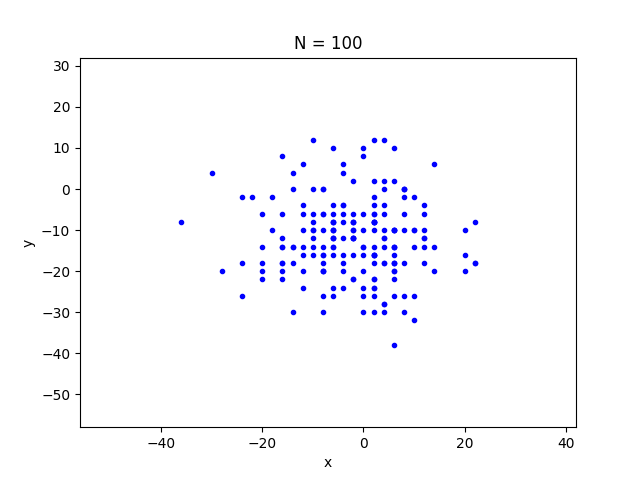
\includegraphics[scale=0.7]{n100.eps}
 \caption{$N=100$}
 \label{n100}
\end{figure}

\begin{figure}[htbp]
 \centering
 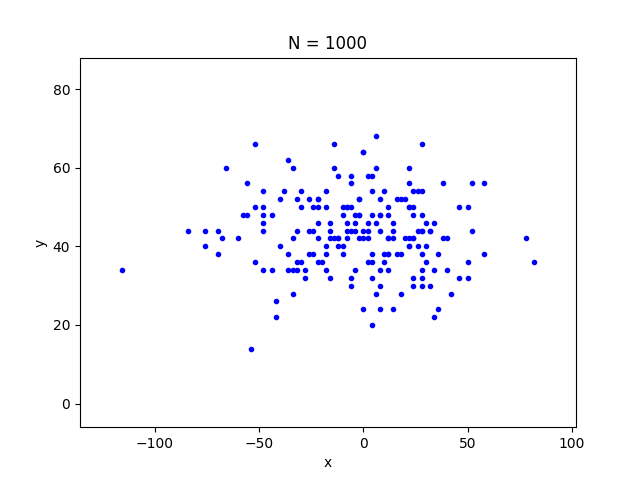
\includegraphics[scale=0.7]{n1000.eps}
 \caption{$N=1000$}
 \label{n103}
\end{figure}

\begin{figure}[htbp]
 \centering
 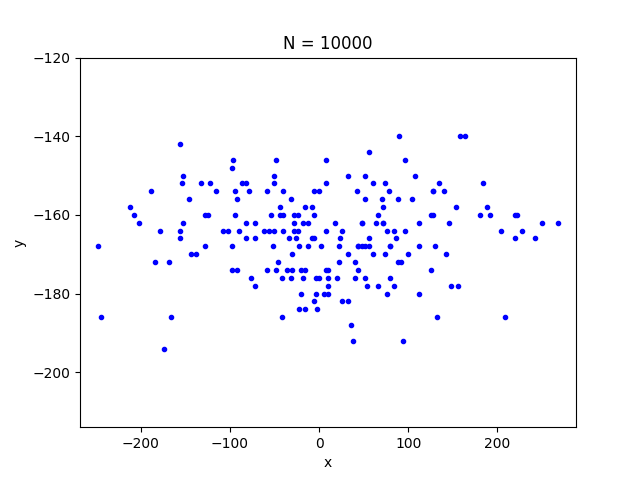
\includegraphics[scale=0.7]{n10000.eps}
 \caption{$N=10000$}
 \label{n104}
\end{figure}

\begin{figure}[htbp]
 \centering
 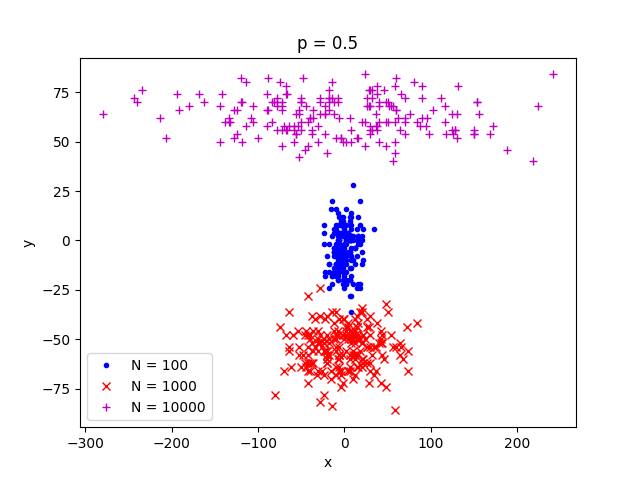
\includegraphics[scale=0.7]{res122_50.eps}
 \caption{$N=100,1000,10000(p=0.5)$}
 \label{nall}
\end{figure}

\begin{figure}[htbp]
 \centering
 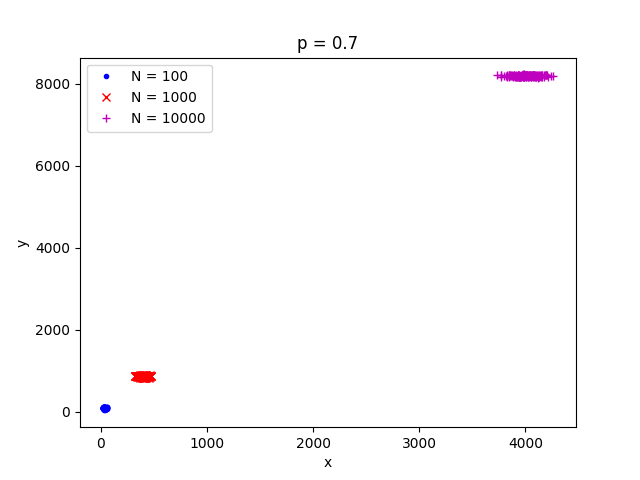
\includegraphics[scale=0.7]{res122_70.eps}
 \caption{$N=100,1000,10000(p=0.7)$}
 \label{nall70}
\end{figure}

図\ref{nall}ではNが増えるにつれて,粒子がちらばっていく様子がわかる.
これは$N$が増えれば増えるほどx,y座標が正の方向に動いた回数と,
負の方向に動いた回数が粒子ごとに異なっていくためであると考えられる.
$p=0.7$の場合は正の方向に動きやすいため,同じ$N$の粒子の集団がどんどん離れていっている.
図\ref{nall70}ではわかりづらいが,左下の点の集まりから順に$N=100,1000,10000$
となっている.

%\begin{figure}[htbp]
%\centering
%\includegraphics[scale=1]{.eps}
%\caption{}
%\label{}
%\end{figure}

\begin{thebibliography}{9}
%\cite{}
% 本:著者(発行年)題名(訳者)発行会社
% web:題名,著者,url,(参照本:著者(発行年)題名(訳者)発行会社 
 \bibitem{sim}栗原正仁(2014)『わかりやすい数値計算入門』ムイスリ出版
\end{thebibliography}

\end{document}